
%!TEX root=../../main.tex

%\begin{doublespace}


\chapter{Distributions of random variables}
\label{modeling}

\index{distribution!normal|(}

%_________________
\section{Normal distribution}
\label{normalDist}

Among the many distributions seen in practice, one is by far the most common: the symmetric, unimodal bell curve. It is often known as the \term{normal curve} or \termsub{normal distribution}{distribution!normal}. Many variables are nearly normal, which makes the normal distribution useful for a variety of problems. For example, characteristics such as human height closely follow the normal distribution.

\begin{figure}
\centering
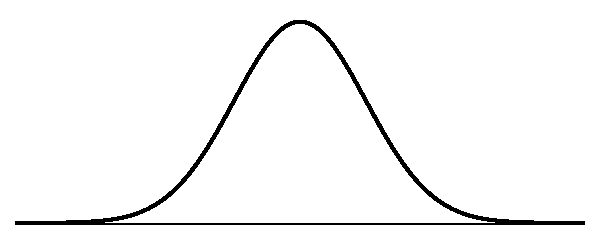
\includegraphics[width=0.7\textwidth]{ch_distributions_oi_biostat/figures/simpleNormal/simpleNormal}
\caption{A normal curve.}
\label{simpleNormal}
\end{figure}

\subsection{Normal distribution model}

The normal distribution model always describes a symmetric, unimodal, bell-shaped curve. However, the curves can differ in center and spread; the model can be adjusted using mean and standard deviation. Changing the mean shifts the bell curve to the left or the right, while changing the standard deviation stretches or constricts the curve. Figure~\ref{twoSampleNormals} shows the normal distribution with mean $0$ and standard deviation $1$ in the left panel and the normal distributions with mean $19$ and standard deviation $4$ in the right panel. Figure~\ref{twoSampleNormalsStacked} shows these distributions on the same axis.

\begin{figure}[hht]
\centering
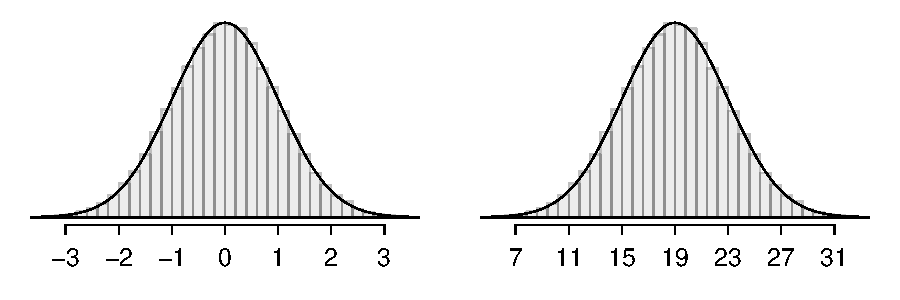
\includegraphics[width=0.85\textwidth]{ch_distributions_oi_biostat/figures/twoSampleNormals/twoSampleNormals}
\caption{Both curves represent the normal distribution; however, they differ in their center and spread. The normal distribution with mean 0 and standard deviation 1 is called the \term{standard normal distribution}.}
\label{twoSampleNormals}
\end{figure}

\begin{figure}[hht]
\centering
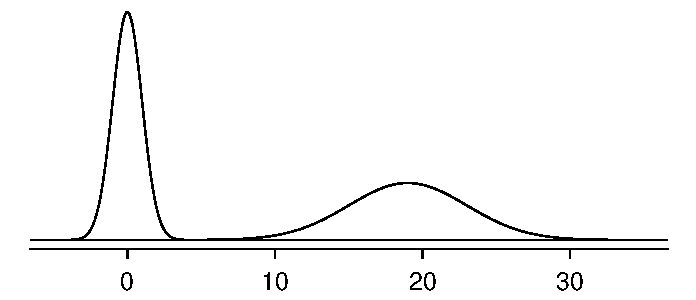
\includegraphics[width=0.6\textwidth]{ch_distributions_oi_biostat/figures/twoSampleNormalsStacked/twoSampleNormalsStacked}
\caption{The normal models shown in Figure~\ref{twoSampleNormals} but plotted together and on the same scale.}
\label{twoSampleNormalsStacked}
\end{figure}

For any given normal distribution with mean $\mu$ and standard deviation $\sigma$, the distribution can be written as $N(\mu, \sigma)$\marginpar[\raggedright\vspace{-5mm}

$N(\mu, \sigma)$\vspace{1mm}\\\footnotesize Normal dist.\\with mean $\mu$\\\& st. dev. $\sigma$]{\raggedright\vspace{-5mm}

$N(\mu, \sigma)$\vspace{1mm}\\\footnotesize Normal dist.\\with mean $\mu$\\\& st. dev. $\sigma$}. For example, $N(0, 1)$ refers to the standard normal distribution, as shown in Figure~\ref{twoSampleNormals}. The mean and standard deviation are the distribution's \termsub{parameters}{parameter}, as they are quantities that precisely define any normal distribution.

\begin{exercise}
Write down the short-hand for a normal distribution with\footnote{(a)~$N(5,3)$. (b)~$N(-100, 10)$. (c)~$N(2, 9)$.}
\begin{parts}
\item mean~5 and standard deviation~3,
\item mean~-100 and standard deviation~10, and
\item mean~2 and standard deviation~9.
\end{parts}
\end{exercise}

\subsection{Standardizing with Z-scores}

The \term{Z-score}\marginpar[\raggedright\vspace{-3mm}

$Z$\vspace{1mm}\\\footnotesize Z-score, the\\standardized\\observation]{\raggedright\vspace{-3mm}
	
	$Z$\vspace{1mm}\\\footnotesize Z-score, the\\standardized\\observation}\index{Z@$Z$} of an observation is defined as the number of standard deviations it falls above or below the mean. If $x$ is an observation from a distribution $N(\mu, \sigma)$, the Z-score is mathematically defined as:
\begin{align*}
	Z = \frac{x-\mu}{\sigma}
\end{align*}

An observation equal to the mean has a Z-score of 0. Observations above the mean have positive Z-scores, while observations below the mean have negative Z-scores. For example, if an observation is one standard deviation above the mean, it has a Z-score of 1; if it is 1.5 standard deviations below the mean, its Z-score is -1.5. 

Z-scores can be used to identify which observations are more extreme than others, and are especially useful when comparing observations from different normal distributions. A Z-score can be plotted on a standard normal curve ($\mu$ = 0, $\sigma$ = 1). One observation $x_1$ is said to be more unusual than another observation $x_2$ if the absolute value of its Z-score is larger than the absolute value of the other observation's Z-score: $|Z_1| > |Z_2|$. In other words, the further an observation is from the mean in either direction, the more extreme it is. 

\begin{example}{The SAT and the ACT are two standardized tests commonly used for college admissions in the United States. The distribution of test scores are both nearly normal. For the SAT, $N(1500, 300)$; for the ACT, $N(21, 5)$. While some colleges request that students submit scores from both tests, others allow students the choice of either the ACT or the SAT. Suppose that one student scores an 1800 on the SAT (Student A) and another scores a 24 on the ACT (Student B). A college admissions officer would like to compare the scores of the two students to determine which student performed better.}\label{actSAT}
		
Calculate a Z-score for each student; i.e., convert $x$ to Z.
		
Using $\mu_{SAT}=1500$, $\sigma_{SAT}=300$, and $x_{A}=1800$, find Student A's Z-score:
\begin{align*}
	Z_{A} = \frac{x_{A} - \mu_{SAT}}{\sigma_{SAT}} = \frac{1800-1500}{300} = 1
\end{align*}

For Student B:
\begin{align*}
	Z_{B} = \frac{x_{B} - \mu_{ACT}}{\sigma_{ACT}} = \frac{24 - 21}{5} = 0.6
\end{align*}

Student A's score is 1 standard deviation above average on the SAT, while Student B's score is 0.6 standard deviations above the mean on the ACT. As illustrated in Figure~\ref{satActNormals}, Student A's score is more extreme, indicating that Student A has scored higher with respect to other scores than Student B.
\end{example}

\begin{figure}[h]
\centering
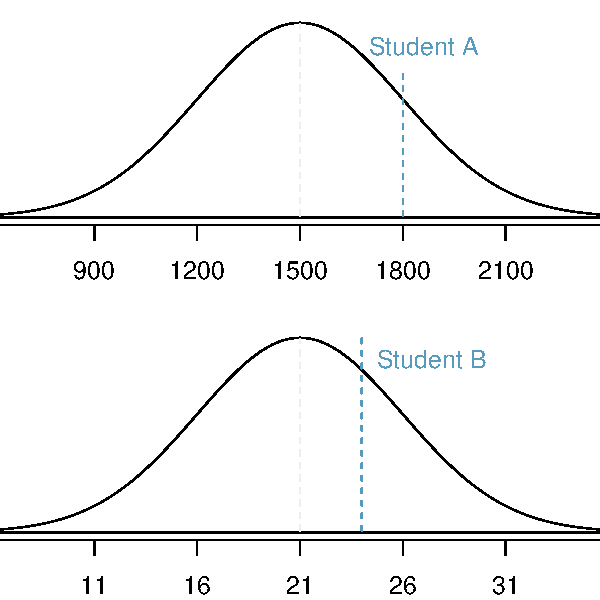
\includegraphics[width=65mm]{ch_distributions_oi_biostat/figures/satActNormals/satActNormals}
\caption{Scores of Students A and B plotted on the distributions of SAT and ACT scores.}
\label{satActNormals}
\end{figure}

\begin{termBox}{\tBoxTitle{The Z-score}
The Z-score of an observation is the number of standard deviations it falls above or below the mean. The Z-score for an observation $x$ that follows a distribution with mean $\mu$ and standard deviation $\sigma$ can be calculated using
\begin{align*}
Z = \frac{x-\mu}{\sigma}
\end{align*}}
\end{termBox}

\begin{example}
{How high would a student need to score on the ACT to have a score equivalent to Student A's score of 1800 on the SAT?} 

As shown in Example~\ref{satActNormals}, a score of 1800 on the SAT is 1 standard deviation above the mean. ACT scores are normally distributed with mean 21 and standard deviation 5. To convert a value from the standard normal curve (Z) to one on a normal distribution $N(\mu, \sigma)$:

\begin{align*}
x = \mu + Z\sigma
\end{align*}

Thus, a student would need a score of $21 + 1(5) = 26$ on the ACT to have a score equivalent to 1800 on the SAT. 
\end{example}

\begin{exercise} \label{nhanes_bp}
Systolic blood pressure (SBP) for adults in the United States aged 18-39 follow an approximate normal distribution, $N(115, 17.5)$. As age increases, systolic blood pressure also tends to increase. Mean systolic blood pressure for adults 60 years of age and older is 136 mm Hg, with standard deviation 40 mm Hg. Systolic blood pressure of 140 mm Hg or higher is indicative of hypertension (high blood pressure). 
(a) How many standard deviations away from the mean is a 30-year-old with systolic blood pressure of 125 mm Hg? (b) Compare how unusual a systolic blood pressure of 140 mm Hg is for a 65-year-old, versus a 30-year-old.\footnote{(a) For $x_1=140$ mm Hg: $Z_1 = \frac{x_1 - \mu}{\sigma} = \frac{140 - 115}{17.5} = 1.43$. (b) For $x_1=140$ mm Hg: $Z_2 = \frac{x_2 - \mu}{\sigma} = \frac{140 - 137}{40} = 0.1$. While an SBP of 140 mm Hg is almost 1.5 standard deviations above the mean for a 30-year-old, it is only 0.1 standard deviations above the mean for a 65-year-old.}
\end{exercise} 

% cite nhanes_bp, SD calculated as SE * sqrt(n) from tables

\subsection{Calculating normal probabilities}

The normal curve is a continuous probability distribution. Recall from Section~\ref{contDist} that the total area under the density curve is always equal to 1, and the probability that a variable has a value within a specified interval is the area under the curve over that interval. By using either statistical software or normal probability tables, the normal model can be used to identify a probability or percentile based on the corresponding Z-score (and vice versa). 

\begin{figure}
	\centering
	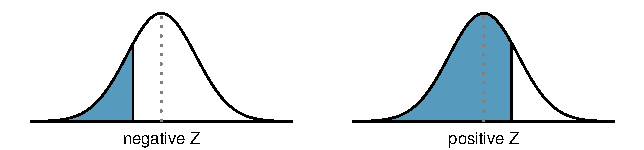
\includegraphics[width=0.9\textwidth]{ch_distributions_oi_biostat/figures/normalTails/normalTails}
	\caption{The area to the left of $Z$ represents the percentile of the observation.}
	\label{normalTails}
\end{figure}

A \term{normal probability table} is given in Appendix~\vref{normalProbabilityTable} and abbreviated in Table~\ref{zTableShort}. This table can be used to identify the \term{percentile} corresponding to any particular Z-score; for instance, the percentile of $Z=0.43$ is shown in row $0.4$ and column $0.03$ in Table~\ref{zTableShort}: 0.6664, or the $66.64^{th}$ percentile. First, find the proper row in the normal probability table up through the first decimal, and then determine the column representing the second decimal value. The intersection of this row and column is the percentile of the observation. This value also represents the probability that the standard normal variable Z takes on a value of 0.43 or less; i.e. $P(Z \leq 0.43) = 0.6664$.

The table can also be used to find the Z-score associated with a percentile. For example, to identify Z for the $80^{th}$ percentile, look for the value closest to 0.8000 in the middle portion of the table: 0.7995. The Z-score for the $80^{th}$ percentile is given by combining the row and column Z values: 0.84.

\begin{table}
	\centering
	\begin{tabular}{c | rrrrr | rrrrr |}
		\cline{2-11}
		&&&& \multicolumn{4}{c}{Second decimal place of $Z$} &&& \\
		\cline{2-11}
		$Z$ & 0.00 & 0.01 & 0.02 & \highlightT{0.03} & \highlightO{0.04} & 0.05 & 0.06 & 0.07 & 0.08 & 0.09 \\
		\hline
		\hline
		0.0 & \scriptsize{0.5000} & \scriptsize{0.5040} & \scriptsize{0.5080} & \scriptsize{0.5120} & \scriptsize{0.5160} & \scriptsize{0.5199} & \scriptsize{0.5239} & \scriptsize{0.5279} & \scriptsize{0.5319} & \scriptsize{0.5359} \\
		0.1 & \scriptsize{0.5398} & \scriptsize{0.5438} & \scriptsize{0.5478} & \scriptsize{0.5517} & \scriptsize{0.5557} & \scriptsize{0.5596} & \scriptsize{0.5636} & \scriptsize{0.5675} & \scriptsize{0.5714} & \scriptsize{0.5753} \\
		0.2 & \scriptsize{0.5793} & \scriptsize{0.5832} & \scriptsize{0.5871} & \scriptsize{0.5910} & \scriptsize{0.5948} & \scriptsize{0.5987} & \scriptsize{0.6026} & \scriptsize{0.6064} & \scriptsize{0.6103} & \scriptsize{0.6141} \\
		%  May comment out 0.0-0.2 to make extra space. Then insert the following line:
		%  $\vdots$ &   $\vdots$ &   $\vdots$ &   $\vdots$ &   $\vdots$ &   $\vdots$ &   $\vdots$ &   $\vdots$ &   $\vdots$ &   $\vdots$ &   $\vdots$ \\
		0.3 & \scriptsize{0.6179} & \scriptsize{0.6217} & \scriptsize{0.6255} & \scriptsize{0.6293} & \scriptsize{0.6331} & \scriptsize{0.6368} & \scriptsize{0.6406} & \scriptsize{0.6443} & \scriptsize{0.6480} & \scriptsize{0.6517} \\
		\highlightT{0.4} & \scriptsize{0.6554} & \scriptsize{0.6591} & \scriptsize{0.6628} & \highlightT{\scriptsize{0.6664}} & \scriptsize{0.6700} & \scriptsize{0.6736} & \scriptsize{0.6772} & \scriptsize{0.6808} & \scriptsize{0.6844} & \scriptsize{0.6879} \\
		\hline
		0.5 & \scriptsize{0.6915} & \scriptsize{0.6950} & \scriptsize{0.6985} & \scriptsize{0.7019} & \scriptsize{0.7054} & \scriptsize{0.7088} & \scriptsize{0.7123} & \scriptsize{0.7157} & \scriptsize{0.7190} & \scriptsize{0.7224} \\
		0.6 & \scriptsize{0.7257} & \scriptsize{0.7291} & \scriptsize{0.7324} & \scriptsize{0.7357} & \scriptsize{0.7389} & \scriptsize{0.7422} & \scriptsize{0.7454} & \scriptsize{0.7486} & \scriptsize{0.7517} & \scriptsize{0.7549} \\
		0.7 & \scriptsize{0.7580} & \scriptsize{0.7611} & \scriptsize{0.7642} & \scriptsize{0.7673} & \scriptsize{0.7704} & \scriptsize{0.7734} & \scriptsize{0.7764} & \scriptsize{0.7794} & \scriptsize{0.7823} & \scriptsize{0.7852} \\
		\highlightO{0.8} & \scriptsize{0.7881} & \scriptsize{0.7910} & \scriptsize{0.7939} & \scriptsize{0.7967} & \highlightO{\scriptsize{0.7995}} & \scriptsize{0.8023} & \scriptsize{0.8051} & \scriptsize{0.8078} & \scriptsize{0.8106} & \scriptsize{0.8133} \\
		0.9 & \scriptsize{0.8159} & \scriptsize{0.8186} & \scriptsize{0.8212} & \scriptsize{0.8238} & \scriptsize{0.8264} & \scriptsize{0.8289} & \scriptsize{0.8315} & \scriptsize{0.8340} & \scriptsize{0.8365} & \scriptsize{0.8389} \\
		\hline
		\hline
		1.0 & \scriptsize{0.8413} & \scriptsize{0.8438} & \scriptsize{0.8461} & \scriptsize{0.8485} & \scriptsize{0.8508} & \scriptsize{0.8531} & \scriptsize{0.8554} & \scriptsize{0.8577} & \scriptsize{0.8599} & \scriptsize{0.8621} \\
		1.1 & \scriptsize{0.8643} & \scriptsize{0.8665} & \scriptsize{0.8686} & \scriptsize{0.8708} & \scriptsize{0.8729} & \scriptsize{0.8749} & \scriptsize{0.8770} & \scriptsize{0.8790} & \scriptsize{0.8810} & \scriptsize{0.8830} \\
		$\vdots$ &   $\vdots$ &   $\vdots$ &   $\vdots$ &   $\vdots$ &   $\vdots$ &   $\vdots$ &   $\vdots$ &   $\vdots$ &   $\vdots$ &   $\vdots$ \\
		\hline
	\end{tabular}
	\caption{A section of the normal probability table. The percentile for a normal random variable with $Z=0.43$ has been \highlightT{highlighted}, and the percentile closest to 0.8000 has also been \highlightO{highlighted}.}
	\label{zTableShort}
\end{table}

\begin{example}{Student A from Example~\ref{actSAT} earned a score of 1800 on the SAT, which corresponds to $Z=1$. What percentile is this score associated with?}
In this context, the \term{percentile} is the percentage of people who earned a lower SAT score than Student A. From the normal table, $Z$ of 1.00 is 0.8643. Thus, the student is in the $86^{th}$ percentile of test takers. This area is shaded in Figure~\ref{satBelow1800}.
\end{example}

\begin{figure}[htb]
   \centering
   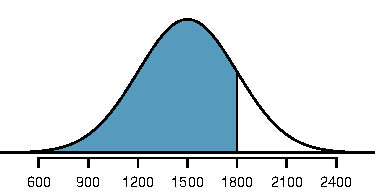
\includegraphics[width=0.6\textwidth]{ch_distributions_oi_biostat/figures/satBelow1800/satBelow1800}
   \caption{The normal model for SAT scores, with shaded area representing scores below 1800.}
   \label{satBelow1800}
\end{figure}

\begin{exercise}
Determine the proportion of SAT test takers who scored better than Student A on the SAT.\footnote{If 84\% had lower scores than Student A, the number of people who had better scores must be 16\%.}
\end{exercise}

\subsection{Normal probability examples}

There are two main types of problems that involve the normal distribution: calculating probabilities from a given value (whether $X$ or $Z$), or identifying the observation that correspond to a particular probability. 

\begin{example}{Cumulative SAT scores are well-approximated by a normal model, $N(1500, 300)$. What is the probability that a randomly selected test taker scores at least 1630 on the SAT?}\label{satAbove1630Exam}
	
For any normal probability problem, it can be helpful to start out by drawing the normal curve and shading the area of interest.

\begin{center}
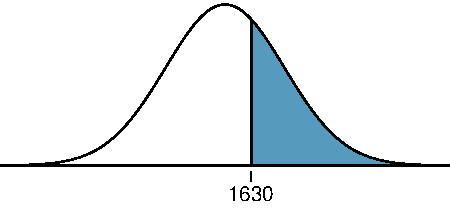
\includegraphics[width=0.45\textwidth]{ch_distributions_oi_biostat/figures/satAbove1630/satAbove1630}
\end{center}
To find the shaded area under the curve, convert 1630 to a Z-score. With $\mu=1500$, $\sigma=300$, and the cutoff value $x=1630$, the Z-score is computed as:
\begin{align*}
Z = \frac{x - \mu}{\sigma} = \frac{1630 - 1500}{300} = \frac{130}{300} = 0.43
\end{align*}
Look up the percentile of $Z=0.43$ in the normal probability table shown in Table~\ref{zTableShort} or in Appendix~\vref{normalProbabilityTable}: 0.6664. However, note that the percentile describes those who had a Z-score \emph{lower} than 0.43, or in other words, the area below 0.43. To find the area \emph{above} $Z=0.43$, subtract the area of the lower tail from the total area under the curve, 1:
\begin{center}
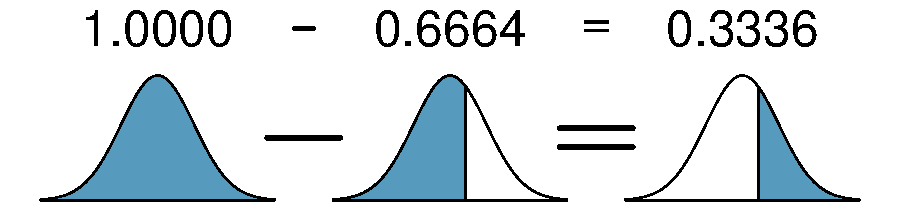
\includegraphics[width=0.5\textwidth]{ch_distributions_oi_biostat/figures/subtractingArea/subtractingArea}
\end{center}
The probability that a student scores at least 1630 on the SAT is 0.3336.
\end{example}


\begin{exercise}
What is the probability of a student scoring at most 1630 on the SAT?\footnote{This probability was calculated as part of Example~\ref{satAbove1630Exam}: 0.6664. A picture for this exercise is represented by the shaded area below ``0.6664'' in Example~\ref{satAbove1630Exam}.}
\end{exercise}

\begin{exercise}
Systolic blood pressure for adults 60 years of age and older in the United States is approximately normally distributed: $N(136, 40)$. What is the probability of an adult in this age group having systolic blood pressure of 140 mm Hg or greater?\footnote{The Z-score for this observation was calculated in Exercise~\ref{nhanes_bp} as 0.1. From the table, this corresponds to 0.54.}
\end{exercise}

\begin{example}{The height of adult males in the United States between the ages of 20 and 62 is nearly normal, with mean 70 inches and standard deviation 3.3 inches.\footnote{As based on a sample of 100 men, from the USDA Food Commodity Intake Database.} What is the probability that a random adult male is between 5'9'' and 6'2''?}
	These heights correspond to 69 inches and 74 inches. First, draw the figure. The area of interest is no longer an upper or lower tail.\textC{\vspace{-2mm}}
	\begin{center}
		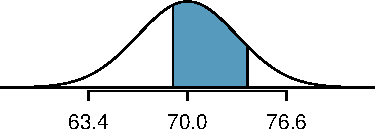
\includegraphics[width=0.35\textwidth]{ch_distributions_oi_biostat/figures/between59And62/between59And62}\textC{\vspace{-2mm}}
	\end{center}
	To find the middle area, find the area to the left of 74; from that area, subtract the area to the left of 69.
	
	First, convert to Z-scores:
	
	\begin{align*}
	Z_{74} = \dfrac{x-\mu}{\sigma} = \dfrac{74-70}{3.3} = 1.21 \qquad Z_{62} = \dfrac{x-\mu}{\sigma} = \dfrac{69-70}{3.3} = -0.30
	\end{align*}
	
	From the normal probability table, the areas are respectively, $0.8868$ and $0.3821$. The middle area is $0.8868 - 0.3821 = 0.5048$. The probability of being between heights 5'9'' and 6'2'' is 0.5048.
\textC{\vspace{-2mm}}
	\begin{center}
		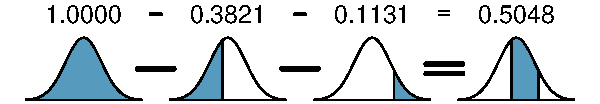
\includegraphics[width=0.6\textwidth]{ch_distributions_oi_biostat/figures/subtracting2Areas/subtracting2Areas}\textC{\vspace{-2mm}}
	\end{center}

\end{example}

\begin{exercise}
	What percentage of adults in the United States ages 60 and older have blood pressure between 145 and 130 mm Hg?\footnote{First calculate Z-scores, then find the percent below 145 mm Hg and below 130 mm Hg: $Z_{145} = 0.23 \to 0.5890$, $Z_{130} = -0.15 \to 0.4404$ (area above). Final answer: $0.5890 - 0.4404 = 0.1486$.}
\end{exercise}

\begin{example}{How tall is a man with height in the 40$^{th}$ percentile?}\label{normalExam40Perc}
First, draw a picture. The lower tail probability is 0.40, so the shaded area must start before the mean. \vspace{-1mm}
\begin{center}
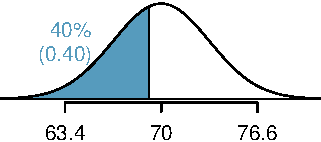
\includegraphics[width=0.35\textwidth]{ch_distributions_oi_biostat/figures/height40Perc/height40Perc}\vspace{-1mm}
\end{center}

Determine the Z-score associated with the $40^{th}$ percentile. Because the percentile is below 50\%, $Z$ will be negative. Look for the probability inside the negative part of table that is closest to 0.40: 0.40 falls in row $-0.2$ and between columns $0.05$ and $0.06$. Since it falls closer to $0.05$, choose $Z=-0.25$.

Convert the Z-score to $X$, where $X \sim N(70, 3.3)$. 

\begin{align*}
X = \mu + \sigma Z = 70 + (-0.25)(3.3) = 69.18
\end{align*}

A man with height in the 40$^{th}$ percentile is 69.18 inches tall, or about 5' 9''. 
\end{example}

\begin{exercise}
(a) What is the $95^{th}$ percentile for SAT scores? (b) What is the $97.5^{th}$ percentile of the male heights? \footnote{(a) Look for 0.95 in the probability portion (middle part) of the normal probability table: row 1.6 and (about) column 0.05, i.e. $Z_{95}=1.65$. Knowing $Z_{95}=1.65$, $\mu = 1500$, and $\sigma = 300$, convert Z to $x$: $1500 + (1.65)(300) = 1995$. (b) Similarly, find $Z_{97.5} = 1.96$, and convert to $x$: $x_{97.5} = 76.5$ inches.}
\end{exercise}

\subsection{The empirical rule}

The empirical rule (also known as the 68-95-99.7 rule) states that for a normal distribution, almost all observations will fall within three standard deviations of the mean. Specifically, 68\% of observations are within one standard deviation of the mean, 95\% are within two SD's, and 99.7\% are within three SD's. This rule can be useful for making quick estimates without using a probability table.

\begin{figure}[hht]
\centering
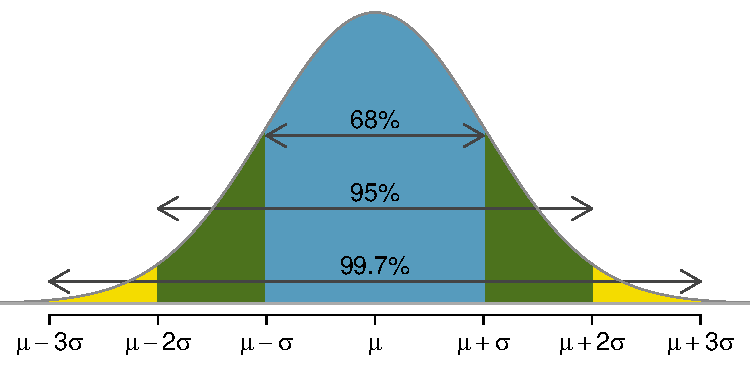
\includegraphics[height=1.9in]{ch_distributions_oi_biostat/figures/6895997/6895997}
\caption{Probabilities for falling within 1, 2, and 3 standard deviations of the mean in a normal distribution.}
\label{6895997}
\end{figure}

While it is possible for a normal random variable to take on values 4, 5, or even more standard deviations from the mean, these occurrences are extremely rare if the data are nearly normal. For example, the probability of being further than 4 standard deviations from the mean is about 1-in-30,000.

\begin{comment}

%_________________
\section{Evaluating the normal approximation}
\label{assessingNormal}

Many processes can be well approximated by the normal distribution. We have already seen two good examples: SAT scores and the heights of US adult males. While using a normal model can be extremely convenient and helpful, it is important to remember normality is always an approximation. Testing the appropriateness of the normal assumption is a key step in many data analyses.

\index{normal probability plot|(}

Example~\ref{normalExam40Perc} suggests the distribution of heights of US males is well approximated by the normal model. We are interested in proceeding under the assumption that the data are normally distributed, but first we must check to see if this is reasonable.

There are two visual methods for checking the assumption of normality, which can be implemented and interpreted quickly. The first is a simple histogram with the best fitting normal curve overlaid on the plot, as shown in the left panel of Figure~\ref{fcidMHeights}. The sample mean $\bar{x}$ and standard deviation $s$ are used as the parameters of the best fitting normal curve. The closer this curve fits the histogram, the more reasonable the normal model assumption. Another more common method is examining a \term{normal probability plot},\footnote{Also commonly called a \term{quantile-quantile plot}.} shown in the right panel of Figure~\ref{fcidMHeights}. The closer the points are to a perfect straight line, the more confident we can be that the data follow the normal model.

\begin{figure}
\centering
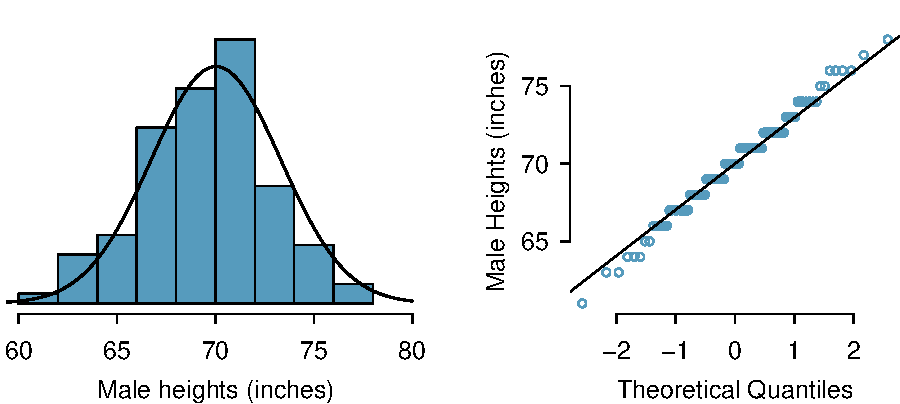
\includegraphics[width=0.8\textwidth]{ch_distributions_oi_biostat/figures/fcidMHeights/fcidMHeights}
\caption{A sample of 100 male heights. The observations are rounded to the nearest whole inch, explaining why the points appear to jump in increments in the normal probability plot.}
\label{fcidMHeights}
\end{figure}

\textC{\newpage}

\begin{example}{Three data sets of 40, 100, and 400 samples were simulated from a normal distribution, and the histograms and normal probability plots of the data sets are shown in Figure~\ref{normalExamples}. These will provide a benchmark for what to look for in plots of real data.} \label{normalExamplesExample}

\begin{figure}
\centering
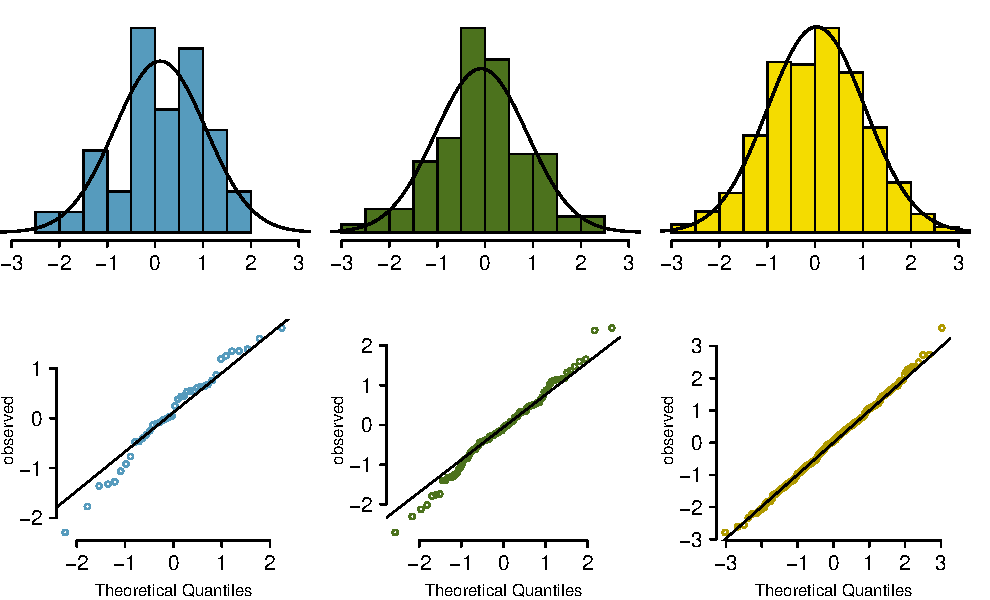
\includegraphics[width=\textwidth]{ch_distributions_oi_biostat/figures/normalExamples/normalExamples}
\caption{Histograms and normal probability plots for three simulated normal data sets; $n=40$ (left), $n=100$ (middle), $n=400$ (right).}
\label{normalExamples}
\end{figure}

The left panels show the histogram (top) and normal probability plot (bottom) for the simulated data set with 40 observations. The data set is too small to really see clear structure in the histogram. The normal probability plot also reflects this, where there are some deviations from the line. We should expect deviations of this amount for such a small data set.

The middle panels show diagnostic plots for the data set with 100 simulated observations. The histogram shows more normality and the normal probability plot shows a better fit. While there are a few observations that deviate noticeably from the line, they are not particularly extreme.

The data set with 400 observations has a histogram that greatly resembles the normal distribution, while the normal probability plot is nearly a perfect straight line. Again in the normal probability plot there is one observation (the largest) that deviates slightly from the line. If that observation had deviated 3 times further from the line, it would be of greater importance in a real data set. Apparent outliers can occur in normally distributed data but they are rare.

Notice the histograms look more normal as the sample size increases, and the normal probability plot becomes straighter and more stable.
\end{example}

\textC{\pagebreak}

\begin{example}{Are NBA player heights normally distributed? Consider all 435 NBA players from the 2008-9 season presented in Figure~\ref{nbaNormal}.\footnote{These data were collected from \oiRedirect{textbook-nba_com}{www.nba.com}.}}
We first create a histogram and normal probability plot of the NBA player heights. The histogram in the left panel is slightly left skewed, which contrasts with the symmetric normal distribution. The points in the normal probability plot do not appear to closely follow a straight line but show what appears to be a ``wave''. We can compare these characteristics to the sample of 400 normally distributed observations in Example~\ref{normalExamplesExample} and see that they represent much stronger deviations from the normal model. NBA player heights do not appear to come from a normal distribution.
\end{example}

\begin{figure}
\centering
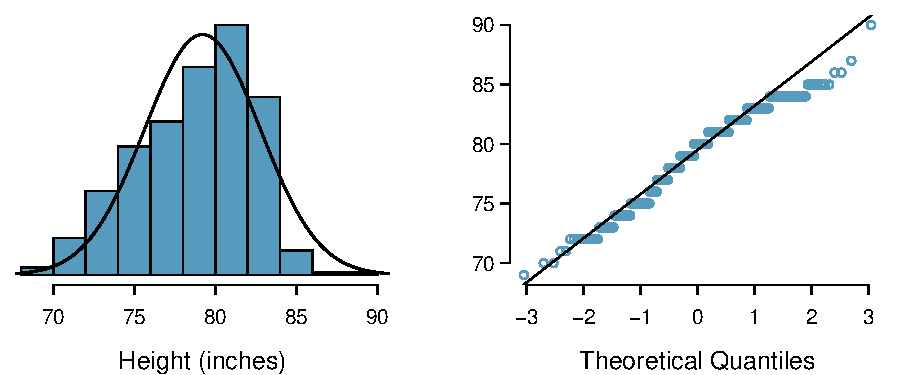
\includegraphics[width=\textwidth]{ch_distributions_oi_biostat/figures/nbaNormal/nbaNormal}
\caption{Histogram and normal probability plot for the NBA heights from the 2008-9 season.}
\label{nbaNormal}
\end{figure}

\begin{example}{Can we approximate poker winnings by a normal distribution? We consider the poker winnings of an individual over 50 days. A histogram and normal probability plot of these data are shown in Figure~\ref{pokerNormal}.}
The data are very strongly right skewed\index{skew!example: very strong} in the histogram, which corresponds to the very strong deviations on the upper right component of the normal probability plot. If we compare these results to the sample of 40 normal observations in Example~\ref{normalExamplesExample}, it is apparent that these data show very strong deviations from the normal model.
\end{example}

\begin{figure}
\centering
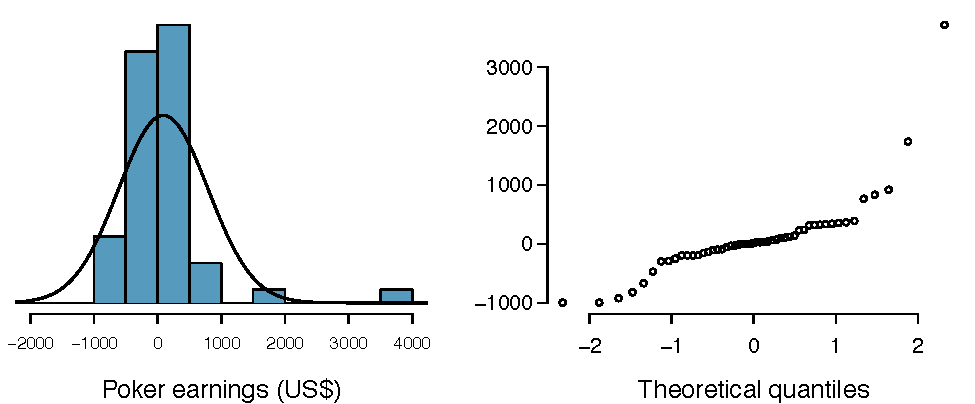
\includegraphics[width=\textwidth]{ch_distributions_oi_biostat/figures/pokerNormal/pokerNormal}
\caption{A histogram of poker data with the best fitting normal plot and a normal probability plot.}
\label{pokerNormal}
\end{figure}

\begin{exercise}\label{normalQuantileExercise}
Determine which data sets represented in Figure~\ref{normalQuantileExer} plausibly come from a nearly normal distribution. Are you confident in all of your conclusions? There are 100 (top left), 50 (top right), 500 (bottom left), and 15 points (bottom right) in the four plots.\footnote{Answers may vary a little. The top-left plot shows some deviations in the smallest values in the data set; specifically, the left tail of the data set has some outliers we should be wary of. The top-right and bottom-left plots do not show any obvious or extreme deviations from the lines for their respective sample sizes, so a normal model would be reasonable for these data sets. The bottom-right plot has a consistent curvature that suggests it is not from the normal distribution. If we examine just the vertical coordinates of these observations, we see that there is a lot of data between -20 and 0, and then about five observations scattered between 0 and 70. This describes a distribution that has a strong right skew.}
\end{exercise}

\begin{figure}
\centering
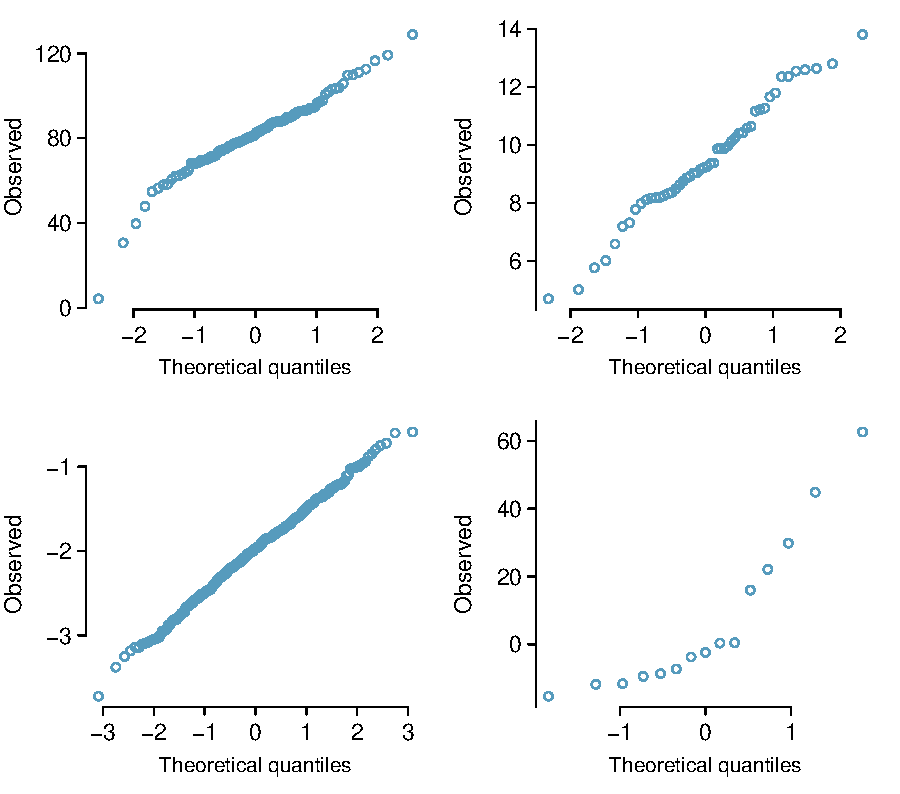
\includegraphics[width=0.9\textwidth]{ch_distributions_oi_biostat/figures/normalQuantileExer/normalQuantileExer}
\caption{Four normal probability plots for Guided Practice~\ref{normalQuantileExercise}.}
\label{normalQuantileExer}
\end{figure}

%When observations spike downwards on the left side of a normal probability plot, it means the data have more outliers in the left tail than we'd expect under a normal distribution. When observations spike upwards on the right side, it means the data have more outliers in the right tail than what we'd expect under the normal distribution.

\begin{exercise} \label{normalQuantileExerciseAdditional}
Figure~\ref{normalQuantileExerAdditional} shows normal probability plots for two distributions that are skewed. One distribution is skewed to the low end (left skewed) and the other to the high end (right skewed). Which is which?\footnote{Examine where the points fall along the vertical axis. In the first plot, most points are near the low end with fewer observations scattered along the high end; this describes a distribution that is skewed to the high end. The second plot shows the opposite features, and this distribution is skewed to the low end.}
\end{exercise}

\begin{figure}
\centering
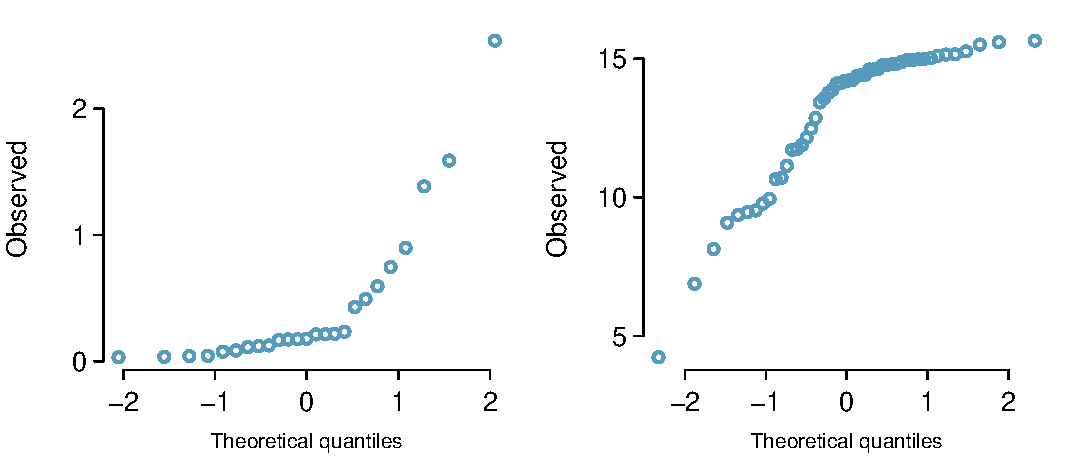
\includegraphics[width=0.9\textwidth]{ch_distributions_oi_biostat/figures/normalQuantileExer/normalQuantileExerAdditional}
\caption{Normal probability plots for Guided Practice~\ref{normalQuantileExerciseAdditional}.}
\label{normalQuantileExerAdditional}
\end{figure}


\index{normal probability plot|)}
\index{distribution!normal|)}

\end{comment}

\textC{\newpage}

\section{Binomial distribution}
\label{binomialModel}

\index{distribution!binomial|(}

\subsection{Bernoulli distribution}
\label{bernoulli}

\index{distribution!Bernoulli|(}

Psychologist Stanley Milgram\index{Milgram, Stanley} began a series of experiments in 1963 to study the effect of authority on obedience. In a typical experiment, a participant would be ordered by an authority figure to give a series of increasingly severe shocks to a stranger. Milgram found that only about 35\% of people would resist the authority and stop giving shocks before the maximum voltage was reached. Over the years, additional research suggested this number is approximately consistent across communities and time.\footnote{Find further information on Milgram's experiment at \par \ \ \hspace{0.2mm}\ \oiRedirect{textbook-milgram}{www.cnr.berkeley.edu/ucce50/ag-labor/7article/article35.htm}.}

Each person in Milgram's experiment can be thought of as a \term{trial}. Suppose that a trial is labeled a \term{success} if the person refuses to administer the worst shock. If the person does administer the worst shock, the trial is a \term{failure}. The \term{probability of a success} can be written as $p=0.35$. The probability of a failure is sometimes denoted with $q=1-p$.

When an individual trial only has two possible outcomes, it is called a \termsub{Bernoulli random variable}{distribution!Bernoulli}. It is arbitrary as to which outcome is labeled success. 

Bernoulli random variables are often denoted as \resp{1} for a success and \resp{0} for a failure. Suppose that ten trials are observed, of which 6 are successes and 4 are failures:
\begin{center}
	\resp{0} \resp{1} \resp{1} \resp{1} \resp{1} \resp{0} \resp{1} \resp{1} \resp{0} \resp{0}
\end{center}
The \term{sample proportion}, $\hat{p}$, is the sample mean of these observations:
\begin{eqnarray*}
	\hat{p} = \frac{\text{\# of successes}}{\text{\# of trials}} = \frac{0+1+1+1+1+0+1+1+0+0}{10} = 0.6
\end{eqnarray*}%
Since \resp{0} and \resp{1} are numerical outcomes, the {mean} and {standard deviation} of a Bernoulli random variable can be defined. If ${p}$ is the true probability of a success, then the mean of a Bernoulli random variable $X$ is given by
	\begin{align*}
	\mu = E[X] &= P(X=0)\times0 + P(X=1)\times1 \\
	&= (1-p)\times0 + p\times 1 = 0+p = p
	\end{align*}
	Similarly, the variance of $X$ can be computed:
	\begin{align*}
	\sigma^2 &= {P(X=0)(0-p)^2 + P(X=1)(1-p)^2} \\
	&= {(1-p)p^2 + p(1-p)^2} = {p(1-p)}
	\end{align*}
	The standard deviation is $\sigma=\sqrt{p(1-p)}$.

\begin{termBox}{\tBoxTitle{Bernoulli random variable}
		If $X$ is a random variable that takes value 1 with probability of success $p$ and 0 with probability $1-p$, then $X$ is a Bernoulli random variable with mean $p$ and standard deviation $\sqrt{p(1-p)}$.
		}
\end{termBox}

\index{distribution!Bernoulli|)}

\begin{example}{Suppose that four individuals are randomly selected to participate in Milgram's experiment. What is the chance that there will be exactly one successful trial? Suppose that the probability of success remains 0.35.}\label{oneRefuser}
	
Consider a scenario in which there is one success (i.e., one person refuses to give the strongest shock). Label the individuals as $A$, $B$, $C$, and $D$:

\begin{align*}
		&P(A=\text{\resp{refuse}},\text{ }B=\text{\resp{shock}},\text{ }C=\text{\resp{shock}},\text{ }D=\text{\resp{shock}}) \\
		&\quad =  P(A=\text{\resp{refuse}})\ P(B=\text{\resp{shock}})\ P(C=\text{\resp{shock}})\ P(D=\text{\resp{shock}}) \\
		&\quad =  (0.35)  (0.65)  (0.65)  (0.65) = (0.35)^1 (0.65)^3 = 0.096
\end{align*}

However, there are three other possible scenarios: either $B$, $C$, or $D$ could have been the one to refuse. In each of these cases, the probability is also $(0.35)^1(0.65)^3$. These four scenarios exhaust all the possible ways that exactly one of these four people could refuse to administer the most severe shock, so the total probability of one success is $4\times(0.35)^1(0.65)^3 = 0.38$.
\end{example}



\subsection{The binomial distribution}

As the simplest of all distributions used to model an experiment, the Bernoulli distribution is unrealistic in all but the simplest of settings. However, it is a useful building block for other distributions. The \termsub{binomial distribution}{distribution!binomial} describes the probability of having exactly $k$ successes in $n$ independent Bernoulli trials with probability of a success $p$. In Example~\ref{oneRefuser}, the goal was to calculate the probability of 1 success out of 4 trials, with probability of success 0.35 ($n=4$, $k=1$, $p=0.35$). 

Unlike the normal distribution, the binomial is a discrete distribution, and can take on only a finite number of values. A binomial variable has values 0, 1, 2, \dots, $n$.

A general formula for the binomial distribution can be developed from re-examining Example~\ref{oneRefuser}. There were four individuals who could have been the one to refuse, and each of these four scenarios had the same probability. Thus, the final probability can be written as:
\begin{eqnarray}
[\text{\# of scenarios}] \times P(\text{single scenario})
\label{genBinomialFormula}
\end{eqnarray}
The first component of this equation is the number of ways to arrange the $k=1$ successes among the $n=4$ trials. The second component is the probability of any of the four (equally probable) scenarios.

Consider $P($single scenario$)$ under the general case of $k$ successes and $n-k$ failures in the $n$ trials. In any such scenario, the Multiplication Rule for independent events can be applied:
\begin{eqnarray*}
	p^k(1-p)^{n-k}
\end{eqnarray*}

Secondly, there is a general formula for the number of ways to choose $k$ successes in $n$ trials, i.e. arrange $k$ successes and $n-k$ failures:
\begin{eqnarray*}
	{n\choose k} = \frac{n!}{k!(n-k)!}
\end{eqnarray*}
The quantity ${n\choose k}$ is read \term{n choose k}.\footnote{Other notation for $n$ choose $k$ includes $_nC_k$, $C_n^k$, and $C(n,k)$.} The exclamation point notation (e.g. $k!$) denotes a \term{factorial}\label{factorialDefinitionInTheBinomialSection} expression.
\begin{eqnarray*}
	&& 0! = 1 \label{zeroFactorial} \\
	&& 1! = 1 \\
	&& 2! = 2\times1 = 2 \\
	&& 3! = 3\times2\times1 = 6 \\
	&& 4! = 4\times3\times2\times1 = 24 \\
	&& \vdots \\
	&& n! = n\times(n-1)\times...\times3\times2\times1
\end{eqnarray*}
Using the formula, the number of ways to choose $k=1$ successes in $n=4$ trials can be computed as:
\begin{eqnarray*}
	{4 \choose 1} = \frac{4!}{1!(4-1)!} =  \frac{4!}{1!3!} 
	= \frac{4\times3\times2\times1}{(1)(3\times2\times1)} = 4
\end{eqnarray*}

Substituting $n$ choose $k$ for the number of scenarios and $p^k(1-p)^{n-k}$ for the single scenario probability in Equation~(\ref{genBinomialFormula}) yields the general binomial formula.

\begin{termBox}{\tBoxTitle{Binomial distribution} Suppose the probability of a single trial being a success is $p$. The probability of observing exactly $k$ successes in $n$ independent trials is given by\vspace{-1mm}
		\begin{eqnarray}
		{n\choose k}p^k(1-p)^{n-k} = \frac{n!}{k!(n-k)!}p^k(1-p)^{n-k}
		\label{binomialFormula}
		\end{eqnarray}
		Additionally, the mean, variance, and standard deviation of the number of observed successes are\vspace{-2mm}
		\begin{align}
		\mu &= np
		&\sigma^2 &= np(1-p)
		&\sigma &= \sqrt{np(1-p)}
		\label{binomialStats}
		\end{align}}
\end{termBox}

\begin{tipBox}{\tipBoxTitle{Is it binomial? Four conditions to check.\label{isItBinomialTipBox}}
		(1) The trials are independent. \\
		(2) The number of trials, $n$, is fixed. \\
		(3) Each trial outcome can be classified as a \emph{success} or \emph{failure}. \\
		(4) The probability of a success, $p$, is the same for each trial.}
\end{tipBox}

\begin{example}{What is the probability that 3 of 8 randomly selected participants will refuse to administer the worst shock?}
	
First, check the conditions for applying the binomial model. The number of trials is fixed ($n=8$) and each trial outcome can be classsified as either success or failure. The sample is random, so the trials are independent, and the probability of success is the same for each trial. 

For the outcome of interest, $k=3$ successes occur in $n=8$ trials, and the probability of a success is $p=0.35$. Thus, the probability that 3 of 8 will refuse is given by
	\begin{eqnarray*}
		P(X =3) = { 8 \choose 3}(0.35)^3(1-0.35)^{8-3}
		&=& \frac{8!}{3!(8-3)!}(0.35)^3(1-0.35)^{8-3} \\
		&=& (56)(0.35)^3(0.65)^5 \\
		&=& 0.28
	\end{eqnarray*}
\end{example}

\begin{example}{What is the probability that at most 3 of 8 randomly selected participants will refuse to administer the worst shock?}

The event of at most 3 out of 8 successes can be thought of as the combined probability of 0, 1, 2, and 3 successes. Thus, the probability that at most 3 of 8 will refuse is given by:
	\begin{align*}
		P(X \leq 3) &= P(X = 0) + P(X = 1) + P(X = 2) + P(X = 3) \\
		&= { 8 \choose 0}(0.35)^0(1-0.35)^{8-0} + { 8 \choose 1}(0.35)^1(1-0.35)^{8-1} \\
		& \qquad + { 8 \choose 2}(0.35)^2(1-0.35)^{8-2} + { 8 \choose 3}(0.35)^3(1-0.35)^{8-3} \\
		&= (1)(0.35)^0(1-0.35)^{8} + (8)(0.35)^1(1-0.35)^{7} \\
		& \qquad + (28)(0.35)^2(1-0.35)^{6} + (56)(0.35)^3(1-0.35)^{5}\\
		&= 0.706
	\end{align*}
\end{example}

\begin{example}{If 40 individuals were randomly selected to participate in the experiment, how many individuals would be expected to refuse to administer the worst shock? What is the standard deviation of the number of people expected to refuse?}

Both quantities can directly be computed from the formulas in Equation~(\ref{binomialStats}). The expected value (mean) is given by: $\mu=np = 40\times 0.35 = 14$. The standard deviation is: $\sigma = \sqrt{np(1-p)} = \sqrt{40\times 0.35\times 0.65} = 3.02$.
\end{example}

\begin{exercise}
The probability that a smoker will develop a severe lung condition in their lifetime is about 0.30. Suppose that 5 smokers are randomly selected from the population. What is the probability that (a) one will develop a severe lung condition? (b) that no more than one will develop a severe lung condition? (c) that at least one will develop a severe lung condition?\footnote{Let the probability of success $p$ equal 0.30. (a) $P(X=1) = {5 \choose 1}(0.30)^1(1-0.30)^{5-1} = 0.36$ (b) $P(X \leq 1) = P(X=0) + P(X=1) = {5 \choose 0}(0.30)^0(1-0.30)^{5-0} + 0.36 = 0.53$ (c) $P(X \geq 1) = 1 - P(X=0) = 1 - 0.36 = 0.83$}	
\end{exercise}

\newpage
	
	\subsection{Normal approximation to the binomial distribution}
	
	\index{distribution!binomial!normal approximation|(}
	
	The binomial formula is cumbersome when the sample size ($n$) is large, particularly when calculating probabilities for a large number of observations. If certain conditions are met, the normal distribution can be used to approximate binomial probabilities. This method is useful when calculating probabilities by hand; however, modern statistical software is capable of calculating exact binomial probabilities even for very large $n$. 
	
	Consider the binomial model when probability of success is $p=0.10$. Figure~\ref{fourBinomialModelsShowingApproxToNormal} shows four hollow histograms for simulated samples from the binomial distribution using four different sample sizes: $n=10, 30, 100, 300$. As the sample size increases from $n=10$ to $n=300$, the distribution is transformed from a blocky and skewed distribution into one resembling the normal curve.
	
	\begin{figure}[h]
		\centering
		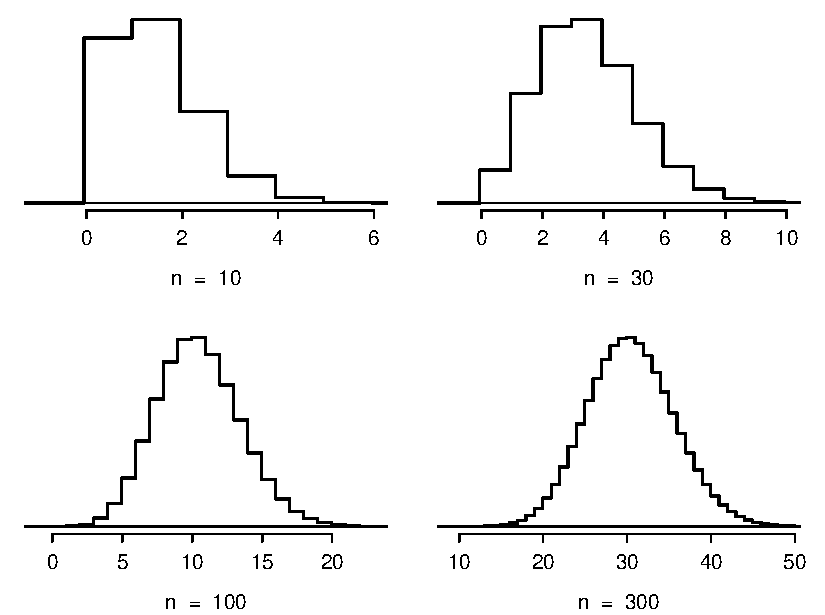
\includegraphics[width=0.92\textwidth]{ch_distributions_oi_biostat/figures/fourBinomialModelsShowingApproxToNormal/fourBinomialModelsShowingApproxToNormal}
		\caption{Hollow histograms of samples from the binomial model when $p=0.10$. The sample sizes for the four plots are $n=10$, 30, 100, and 300, respectively.}
		\label{fourBinomialModelsShowingApproxToNormal}
	\end{figure}
	
	\begin{termBox}{\tBoxTitle{Normal approximation of the binomial distribution}
		The binomial distribution with probability of success $p$ is nearly normal when the sample size $n$ is sufficiently large such that $np$ and $n(1-p)$ are both at least 10. The approximate normal distribution has parameters corresponding to the mean and standard deviation of the binomial distribution:\vspace{-1.5mm}
			\begin{align*}
			\mu &= np
			&&\sigma= \sqrt{np(1-p)}
			\end{align*}}
	\end{termBox}
	
	\begin{example}{Approximately 20\% of the US population smokes cigarettes. A local government commissioned a survey of 400 randomly selected individuals to investigate whether their community might have a lower smoker rate than 20\%. The survey found that 59 of the 400 participants smoke cigarettes. If the true proportion of smokers in the community is 20\%, what is the probability of observing 59 or fewer smokers in a sample of 400 people?}\label{approxBinomialForN400P20SmokerExample}
		
		The desired probability is equivalent to the sum of the individual probabilities of observing $k=0$, 1, ..., 58, or 59 smokers in a sample of $n=400$: $P(X \leq 59)$. Confirm that the normal approximation is valid: $np=400\times 0.20=80$, $n(1-p)=400\times 0.8=320$. To use the normal approximation, calculate the mean and standard deviation from the binomial model:
		
		\begin{align*}
		\mu &= np = 80
		&\sigma &= \sqrt{np(1-p)} = 8
		\end{align*}
		
		Convert 59 to a Z-score: $Z = \dfrac{59-80}{8} = -2.63$. Use the normal probability table to identify the left tail area, which is 0.0043. 
		
		This estimate is very close to the answer derived from the exact binomial calculation:
		\begin{align*}
		&P(k=0\text{ or }k=1\text{ or }\cdots\text{ or } k=59) \\
		&\qquad= P(k=0) + P(k=1) + \cdots + P(k=59) \\
		&\qquad=0.0041
		\end{align*}
	\end{example}

However, even when the conditions for using the approximation are met, the normal approximation to the binomial tends to perform poorly when estimating the probability of a small range of counts. Suppose the normal approximation is used to compute the probability of observing 69, 70, or 71 smokers in 400 when $p=0.20$. In this setting, the exact binomial and normal approximate result in notably different answers: the approximation gives 0.0476, while the binomial returns 0.0703.

The cause of this discrepancy is illustrated in Figure~\ref{normApproxToBinomFail}, which shows the areas representing the binomial probability (outlined) and normal approximation (shaded). Notice that the width of the area under the normal distribution is 0.5 units too slim on both sides of the interval.

	\begin{figure}[h]
		\centering
		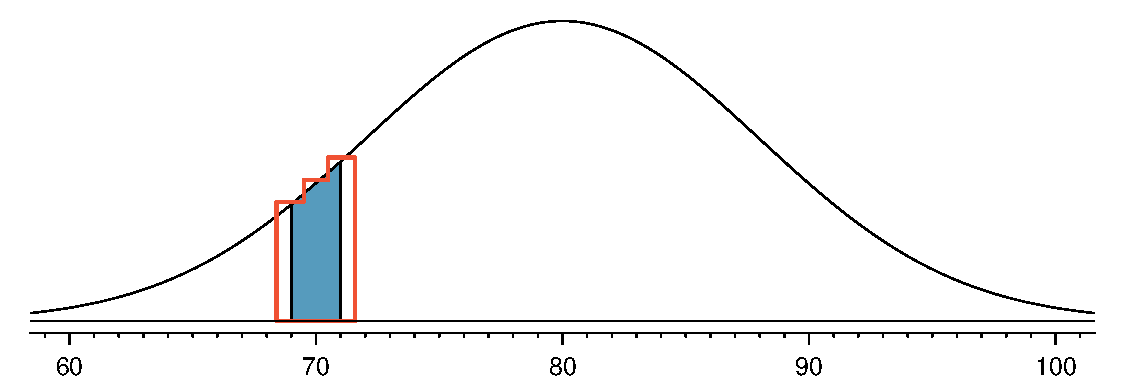
\includegraphics[width=\textwidth]{ch_distributions_oi_biostat/figures/normApproxToBinomFail/normApproxToBinomFail}
		\caption{A normal curve with the area between 69 and 71 shaded. The outlined area represents the exact binomial probability.}
		\label{normApproxToBinomFail}
	\end{figure}
	
The normal approximation can be improved if the cutoff values for the range of observations is modified slightly: the lower value should be reduced by 0.5 and the upper value increased by 0.5. This adjustment method is known as a continuity correction, which allows for increased accuracy when a continuous distribution is used to approximate a discrete one. The modification is typically not necessary when computing a tail area, since the total interval is then typically quite wide.
	
\index{distribution!binomial!normal approximation|)}
\index{distribution!binomial|)}

%_________________
\section{Poisson distribution}
\label{poisson}

\index{distribution!Poisson|(}

The \termsub{Poisson distribution}{distribution!Poisson} is often useful for estimating the number of events in a large population over a unit of time, if the individuals within the population are independent. For example, consider the population of New York City: 8 million individuals. In a given day, how many individuals might be hospitalized for acute myocardial infarction (AMI), i.e., a heart attack? According to historical records, about 4.4 individuals on average. A histogram of the number of occurrences of AMI on 365 days for NYC is shown in Figure~\ref{amiIncidencesOver100Days}.\footnote{These data are simulated. In practice, it would be important to check for an association between successive days.}

\begin{figure}[h]
	\centering
	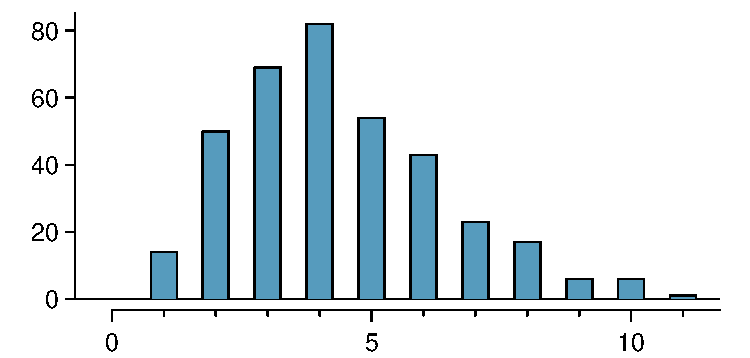
\includegraphics[width=0.7\textwidth]{ch_distributions_oi_biostat/figures/amiIncidencesOver100Days/amiIncidencesOver100Days}
	\caption{A histogram of the number of occurrences of AMI on 365 separate days in NYC.}
	\label{amiIncidencesOver100Days}
\end{figure}

The \term{rate} for a Poisson distribution is the average number of occurrences in a mostly-fixed population per unit of time. The only parameter in the Poisson distribution is the rate, and it is typically denoted by $\lambda$\marginpar[\raggedright\vspace{-5mm}

$\lambda$\vspace{0mm}\\\footnotesize Rate for the\\Poisson dist.]{\raggedright\vspace{-5mm}
	
	$\lambda$\vspace{0mm}\\\footnotesize Rate for the\\Poisson dist.}\index{Greek!lambda@lambda ($\lambda$)}
(the Greek letter \emph{lambda}). Using the rate, we can describe the probability of observing exactly $k$ events in a single unit of time. The histogram in Figure~\ref{amiIncidencesOver100Days} approximates a Poisson distribution with rate equal to 4.4 events in a day, for a population of 8 million. 

\begin{termBox}{\tBoxTitle{Poisson distribution}
		Suppose events occur over time in such a way that the probability an event occurs in an interval is proportional to the length of the interval, and that events occur independently at a rate $\lambda$ per unit of time. Then the probability of exactly $k$ events in $t$ units of time is:

		\begin{align*}
		P(X = k) = \frac{e^{-\lambda t}(\lambda t)^{k}}{k!}
		\end{align*}
		where $k$ may take a value 0, 1, 2, \dots The mean and standard deviation of this distribution are $\lambda$ and $\sqrt{\lambda}$, respectively.}
\end{termBox}

\begin{example}{In New York City, what is the probability that 2 individuals are hospitalized for AMI in seven days, if the rate is known to be 4.4 deaths per day?}

From the given information, $\lambda = 4.4$, $k = 2$, and $t = 7$. 

\begin{align*}
P(X = k) =& \frac{e^{-\lambda t}(\lambda t)^{k}}{k!} \\
P(X = 2) =& \frac{e^{-4.4 \times 7}(4.4 \times 7)^{2}}{2!} \\
=& 1.99 \times 10^{11}
\end{align*}
	
\end{example}

\begin{exercise}
In New York City, what is the probability that (a) at most 2 individuals are hospitalized for AMI in seven days, (b) at least 3 individuals are hospitalized for AMI in seven days?\footnote{(a) $P(X \leq 2) = P(X=0) + P(X=1) + P(X=2) = \frac{e^{-4.4 \times 7}(4.4 \times 7)^{0}}{0!} + \frac{e^{-4.4 \times 7}(4.4 \times 7)^{1}}{1!} + \frac{e^{-4.4 \times 7}(4.4 \times 7)^{2}}{2!} = 2.12 \times 10^{-11}$ (b) $P(X \geq 3) = 1 - P(X < 3) = 1 - P(X \leq 2) = 1 - 2.12 \times 10^{-11} \approx 1 $}
\end{exercise}

A rigorous set of conditions for the Poisson distribution is not discussed here. Generally, the Poisson distribution is used to calculate probabilities for rare events that accumulate over time, such as the occurrence of a disease in a population.

\begin{example}{
For children ages 0 - 14, the incidence rate of acute lymphocytic leukemia (ALL) was approximately 30 diagnosed cases per million children per year in 2010. Approximately 20\% of the US population of 319,055,000 are in this age range. What is the expected number of cases of ALL in the US over five years?}

The incidence rate for one year can be expressed as $30/1,000,000 = 0.00003$; for five years, the rate is $(5)(0.00003) = 0.00015$. The number of children age 0-14 in the population is $(0.20)(319,055,000) \approx 63,811,000$. 

\begin{align*}
\lambda &= \text{(relevant population size)(rate per child)} \\
&= 63,811,000 \times 0.00015 \\
&= 9,571.5
\end{align*}
	
The expected number of cases over five years is 9,571.5 cases.	
	
\end{example}

% example from unit 3 lecture

\index{distribution!Poisson|)}

%_________________
\section{Geometric distribution (special topic)}
\label{geomDist}

\index{distribution!geometric|(}

The geometric distribution describes the waiting time until one success for a series of independent Bernoulli random variables, in which the probability of success $p$ remains constant.

\begin{example}{Recall that in the Milgram shock experiments, the probability of a person refusing to give the most severe shock is $p = 0.35$. Suppose that participants are tested one at a time until one person refuses; i.e., until the first occurrence of a successful trial. What are the chances that the first occurrence happens with the first trial? The second trial? The third?}\label{waitForShocker}
	
The probability that the first trial is successful is simply $p = 0.35$. 

If the second trial is the first successful one, then the first one must have been unsuccessful. Thus, the probability is given by $(0.65)(0.35) = 0.228$.

Similarly, the probability that the first success is the third trial: $(0.65)(0.65)(0.35) = 0.148$.

This can be stated generally. If the first success is on the $n^{th}$ trial, then there are $n-1$ failures and finally 1 success, which corresponds to the probability $(0.65)^{n-1}(0.35)$.
\end{example}

The geometric distribution from Example~\ref{waitForShocker} is shown in Figure~\ref{geometricDist35}. In general, the probabilities for a geometric distribution decrease \term{exponentially}.

\begin{figure}
\centering
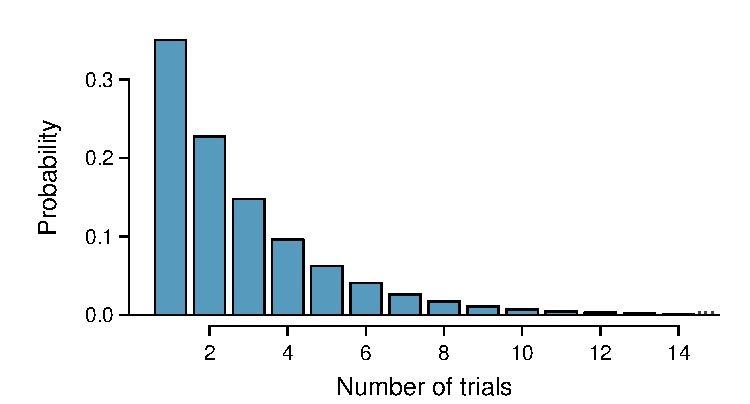
\includegraphics[width=0.8\textwidth]{ch_distributions_oi_biostat/figures/geometricDist35/geometricDist35}
\caption{The geometric distribution when the probability of success is $p=0.35$.}
\label{geometricDist35}
\end{figure}

\begin{termBox}{\tBoxTitle{Geometric Distribution\index{distribution!geometric|textbf}}
If the probability of a success in one trial is $p$ and the probability of a failure is $1-p$, then the probability of finding the first success in the $n^{th}$ trial is given by\vspace{-1.5mm}
\begin{eqnarray}
(1-p)^{n-1}p
\end{eqnarray}
The mean (i.e. expected value), variance, and standard deviation of this wait time are given by\vspace{-2.5mm}
\begin{align}
\mu &= \frac{1}{p}
	&\sigma^2&=\frac{1-p}{p^2}
	&\sigma &= \sqrt{\frac{1-p}{p^2}}
\label{geomFormulas}
\end{align}}
\end{termBox}

\begin{exercise}
If individuals were examined until one did not administer the most severe shock, how many might need to be tested before the first success? \footnote{About $1/p = 1/0.35 = 2.86$ individuals.}
\end{exercise}

\begin{example}{What is the probability of the first success occurring within the first 4 people?} \label{marglimFirstSuccessIn4}
This is the probability it is the first ($n=1$), second ($n=2$), third ($n=3$), or fourth ($n=4$) trial that is the first success, which represent four disjoint outcomes. Compute the probability of each case and add the separate results:
\begin{eqnarray*}
&&P(X=1, 2, 3,\text{ or }4) \\
	&& \quad = P(X=1)+P(X=2)+P(X=3)+P(X=4) \\
	&& \quad = (0.65)^{1-1}(0.35) + (0.65)^{2-1}(0.35) + (0.65)^{3-1}(0.35) + (0.65)^{4-1}(0.35) \\
	&& \quad = 0.82
\end{eqnarray*}

Alternatively, find the complement of P(X = 0), since the described event is the complement of no success in 4 trials: $1 - (0.65)^{4}(0.35)^{0} = 0.82$.

There is a 0.82 probability that the first success occurs within 4 trials.
\end{example}

\index{distribution!geometric|)}



%_________________
\section{Negative binomial distribution (special topic)}
\label{negativeBinomial}

\index{distribution!negative binomial|(}

The geometric distribution describes the probability of observing the first success on the $n^{th}$ trial. The \termsub{negative binomial distribution}{distribution!negative binomial} is more general: it describes the probability of observing the $k^{th}$ success on the $n^{th}$ trial.

Suppose a research assistant needs to successfully extract RNA from four plant samples before leaving the lab for the day. Yesterday, it took 6 attempts to attain the fourth successful extraction. The last extraction must have been a success; that leaves three successful extractions and two unsuccessful ones that make up the first five attempts. There are ten possible sequences, which are shown in \ref{successFailureOrdersForRNAExtractions}. 

\begin{table}[ht]
	\newcommand{\succObs}[1]{{\color{oiB}$\stackrel{#1}{S}$}}
	\centering
	\begin{tabular}{c|c ccc cl | r}
		\multicolumn{8}{c}{\hspace{10mm}Extraction Attempt} \\
		& & 1 & 2 & 3 & 4 & \multicolumn{2}{l}{5\hfill6} \\
		\hline
		1&& $F$ & $F$ & \succObs{1} & \succObs{2} & \succObs{3} & \succObs{4} \\
		2&& $F$ & \succObs{1} & $F$ & \succObs{2} & \succObs{3} & \succObs{4} \\
		3&& $F$ & \succObs{1} & \succObs{2} & $F$ & \succObs{3} & \succObs{4} \\
		4&& $F$ & \succObs{1} & \succObs{2} & \succObs{3} & $F$ & \succObs{4} \\
		5&& \succObs{1} & $F$ & $F$ & \succObs{2} & \succObs{3} & \succObs{4} \\
		6&& \succObs{1} & $F$ & \succObs{2} & $F$ & \succObs{3} & \succObs{4} \\
		7&& \succObs{1} & $F$ & \succObs{2} & \succObs{3} & $F$ & \succObs{4} \\
		8&& \succObs{1} & \succObs{2} & $F$ & $F$ & \succObs{3} & \succObs{4} \\
		9&& \succObs{1} & \succObs{2} & $F$ & \succObs{3} & $F$ & \succObs{4} \\
		10&& \succObs{1} & \succObs{2} & \succObs{3} & $F$ & $F$ & \succObs{4} \\
	\end{tabular}
	\caption{The ten possible sequences when the fourth successful extraction is on the sixth attempt.}
	\label{successFailureOrdersForRNAExtractions}
\end{table}

\begin{exercise} \label{probOfEachSeqOfSixTriesToGetFourSuccesses}
	Each sequence in Table~\ref{successFailureOrdersForRNAExtractions} has exactly two failures and four successes with the last attempt always being a success. If the probability of a success is $p=0.8$, find the probability of the first sequence.\footnote{The first sequence: $0.2\times0.2\times0.8\times0.8\times0.8\times0.8 = 0.0164$.}
\end{exercise}

If the probability of a successful extraction is $p=0.8$, what is the probability that it takes exactly six attempts to reach the fourth successful extraction? As expressed by \ref{probOfEachSeqOfSixTriesToGetFourSuccesses}, there are 10 different ways that this event can occur. The probability of the first sequence was identified in Guided Practice~\ref{probOfEachSeqOfSixTriesToGetFourSuccesses} as 0.0164, and each of the other sequences have the same probability. Thus, the total probability is $(10)(0.0164) = 0.164$.

A general formula for computing a negative binomial probability can be generated using similar logic as for binomial probability. The probability is comprised of two pieces: the probability of a single sequence of events, and then the number of possible sequences. The probability of observing $k$ successes out of $n$ attempts can be expressed as $(1-p)^{n-k} p^{k}$. Next, identify the number of possible sequences. In the above example, 10 sequences were identified by fixing the last observation as a success and looking for ways to arrange the other observations. In other words, the goal is to arrange $k-1$ successes in $n-1$ trials. This can be expressed as: \[{n-1 \choose k-1} = \frac{(n-1)!}{(k-1)! \left((n-1) - (k-1)\right)!} = \frac{(n-1)!}{(k-1)! \left(n - k\right)!}\]

\begin{termBox}{\tBoxTitle{Negative binomial distribution}
		The negative binomial distribution describes the probability of observing the $k^{th}$ success on the $n^{th}$ trial, for independent trials:
		\begin{eqnarray}
		P(\text{the $k^{th}$ success on the $n^{th}$ trial}) = {n-1 \choose k-1} p^{k}(1-p)^{n-k}
		\label{negativeBinomialEquation}
		\end{eqnarray}
		where $p$ is the probability an individual trial is a success.}
\end{termBox}

\begin{tipBox}{\tipBoxTitle{Is it negative binomial? Four conditions to check.}
		(1) The trials are independent. \\
		(2) Each trial outcome can be classified as a success or failure. \\
		(3) The probability of a success ($p$) is the same for each trial. \\
		(4) The last trial must be a success.}
\end{tipBox}


\begin{example}{Show using Equation~\eqref{negativeBinomialEquation} that the probability of a fourth successful extraction on the sixth attempt is 0.164.}
The probability of a single success is $p=0.8$, the number of successes is $k=4$, and the number of necessary attempts under this scenario is $n=6$.
\begin{align*}
{n-1 \choose k-1}p^k(1-p)^{n-k}\ 
	=\ \frac{5!}{3!2!} (0.8)^4 (0.2)^2\ 
	=\ 10\times 0.0164\ 
	=\ 0.164
\end{align*}
\end{example}

\begin{exercise}
Assume that each extraction attempt is independent. What is the probability that the fourth success occurs within 5 attempts?\footnote{If the fourth success ($k=4$) is within five attempts, it either took four or five tries ($n=4$ or $n=5$). Use Equation~\eqref{negativeBinomialEquation} to compute the probability of $n=4$ tries and $n=5$ tries, then add those probabilities together:
\begin{align*}
& P(n=4\text{ OR }n=5) = P(n=4) + P(n=5) \\
&\quad = {4-1 \choose 4-1} 0.8^4 + {5-1 \choose 4-1} (0.8)^4(1-0.8) = 1\times 0.41 + 4\times 0.082 = 0.41 + 0.33 = 0.74
\end{align*}}
\end{exercise}

\begin{tipBox}{\tipBoxTitle{Binomial versus negative binomial}
The binomial distribution is used when considering the number of successes for a fixed number of trials. For negative binomial problems, there is a fixed number of successes and the goal is to identify the number of trials necessary for a certain number of successes (note that the last observation must be a success).}
\end{tipBox}

\begin{exercise}
On 70\% of days, a hospital admits at least one heart attack patient. On 30\% of the days, no heart attack patients are admitted. Identify each case below as a binomial or negative binomial case, and compute the probability. (a) What is the probability the hospital will admit a heart attack patient on exactly three days this week? (b) What is the probability the second day with a heart attack patient will be the fourth day of the week? (c) What is the probability the fifth day of next month will be the first day with a heart attack patient?\footnote{In each part, $p=0.7$. (a) The number of days is fixed, so this is binomial. The parameters are $k=3$ and $n=7$: 0.097. (b) The last "success" (admitting a patient) is fixed to the last day, so apply the negative binomial distribution. The parameters are $k=2$, $n=4$: 0.132. (c) This problem is negative binomial with $k=1$ and $n=5$: 0.006. Note that the negative binomial case when $k=1$ is the same as using the geometric distribution.}
\end{exercise}

\index{distribution!negative binomial|)}

\textC{\pagebreak}

%\end{doublespace}